\documentclass[12pt]{article}
\usepackage{hyperref}
\usepackage{graphicx}
\usepackage{color}
\title{The Variation Toolkit}
\author{Pierre Lindenbaum PhD.
\\
\\Institut du Thorax\\INSERM UMR-915\\44000 Nantes - France\\
\\
\texttt{plindenbaum@yahoo.fr}\\ \url{http://plindenbaum.blogspot.com}\\ \url{https://twitter.com/yokofakun}
\\
}
\date{\today}



\begin{document}
\maketitle

%%\begin{abstract}
%%C++ tools for the interpretations of NGS data.
%%\end{abstract}
\cleardoublepage
\section{Introduction}
The Variation Toolkit is a set of C/C++ programs to handle Variant Call Format (VCF).
The programs have been preliminary designed for knime4bio ( \url{http://code.google.com/p/knime4bio/}) \cite{pmid21984761}
but here, the bioinformaticians are the preliminary audience for this toolkit.
\section{Building}
\subsection{Dependencies}
\begin{description}
\item[Samtools]: Utilities for post-processing alignments in the SAM format. \cite{pmid19505943}
\item[Tabix]: fast retrieval of sequence features from generic TAB-delimited files. \cite{pmid21208982}
\item[mysql-dev]: the files and libraries for mysql.
\item[libxml2]: the C library for xml \url{http://xmlsoft.org/}.
\item[libxslt]: the C library for xslt \url{http://xmlsoft.org/XSLT/}.
\item[libcurl]: the C library for downloading URLs.
\item[jkentsrc]: (optional) Jim Kent's C library / Ucsc parsing bigbed, bigwig...
\end{description}
\subsection{Building}
Download the latest version of varking using \texttt{subversion}:

\begin{quote}
\$ svn checkout http://variationtoolkit.googlecode.com/svn/trunk/ variationtoolkit-read-only
\end{quote}

or update your current version by calling \texttt{"svn update"} in the  variationtoolkit folder.
\begin{quote} 
\$ svn update
\end{quote}

Edit the file variationtoolkit/config.mk . You'll have to set the path to the sources of tabix (>=0.2.5), samtools (>=-0.1.18), etc..

then type:
\begin{quote}
\$ make
\end{quote}
the binaries will be generated in the "bin" folder.

\subsection{Colors}
Some programs use colors (e.g; 'manhattan' ). Colors can be specified as a rgb triple (e.g: 'rgb(100,10,100), rgb(0.5)', as a name (e.g: 'red'), as an hexadecimal '\#AAAAAA', etc...
\subsection{Base index}
The tools reading and writing VCF-like files use '+1' as the index of the first base.
\subsection{Input}
The tools read from files or from the standard input. The streams can be gzipped.

\section{Tools}
All the tools have the option "-h" that provides some help.


\subsection{scanvcf}
Reads a strean with two columns: a Sample-Name and the file path to a VCF(.gz) . It then prints all the VCF, adding an extra column with the sample name to the output.

\paragraph{Options:}
\begin{itemize}
\item--sample or -S (column-index) column for the path to SAMPLE 
\item--vcf or -V (column-index) column for the path to VCF(.gz)
\end{itemize}

\paragraph{Example:}
\begin{quote}
\begin{verbatim}
$ head -n3 input.txt

#Sample	VCF
Sample1	data/sample1.vcf.gz
Sample2	data/sample1.vcf.gz
Sample2	data/sample1.vcf.gz


$ cat input.txt |scanvcf 

#CHROM POS ID REF ALT QUAL FILTER . FORMAT Call SAMPLE
1 879317 rs7523549 C T 71 0 . GT:GQ:DP:FLT 0/1:34:8:0 Sample1
1 880238 rs3748592 A G 51 0 . GT:GQ:DP:FLT 1/1:51:8:0 Sample1
1 880390 rs3748593 C A 99 0 . GT:GQ:DP:FLT 1/0:99:30:0 Sample1
1 881627 rs2272757 G A 99 0 . GT:GQ:DP:FLT 1/0:59:20:0 Sample1
(...)
Y 13524507 . C T 99 0 . GT:GQ:DP:FLT 1/1:99:233:0 Sample20
Y 21154323 rs10465459 G A 99 0 . GT:GQ:DP:FLT 1/1:99:215:0 Sample20
Y 21154426 rs52812045 G A 99 0 . GT:GQ:DP:FLT 1/0:99:143:0 Sample20
Y 21154466 rs10465460 T A 99 0 . GT:GQ:DP:FLT 1/1:99:134:0 Sample20
Y 21154529 . G A 51 0 . GT:GQ:DP:FLT 1/1:51:8:0 Sample20
\end{verbatim}
\end{quote}


\subsection{extractinfo}
Extract a field from the INFO column of a VCF file.
\paragraph{Options:}
\begin{itemize}
\item-c (info-column-infex) (7)
\item--delim (column-delimiter) (default:tab)
\item-t (tag) (required)
\item-N (string) symbol for NOT-FOUND. default:N/A
\item-i ignore line if tag was not found
\end{itemize}
\paragraph{Example:}
The following script extract the GN(gene name) field from the column INFO. We keep the lines for the gene NOTCH2 and we display the associated SNP.
\begin{quote}
\begin{verbatim}
$ gunzip -c data.vcf.gz |\
  extractinfo -t GN -i | \
  awk -F '       ' '($11 =="NOTCH2")' |\
  cut -d ' ' -f 3 | grep rs

rs6685892
rs2493392
rs2493420
rs7534585
rs7534586
rs2493409
rs2453040
rs2124109

\end{verbatim}
\end{quote}

\subsection{extractformat}
Extract a field from the FORMAT column of a VCF file.
\paragraph{Options:}
\begin{itemize}
\item-f (format-column-infex) (8)
\item-c (call-column-infex) (9)
\item--delim (column-delimiter) (default:tab)
\item-t (tag) (required)
\item-N (string) symbol for NOT-FOUND. default:N/A
\end{itemize}
\paragraph{Example:}
The following command line extract the field 'GT' from the VCF and we count the occurence of the values.

\begin{quote}
\begin{verbatim}
$ gunzip -c data.vcf.gz |\
   extractformat -t GT |\
   cut -d '        ' -f 11 |\
   sort |\
    uniq -c

     29 
  10729 0/1
  10800 1/0
  13518 1/1
     11 1/2
\end{verbatim}
\end{quote}

\subsection{ncbiefetch}
Fetch a record from NCBI database.
Currently supported databases: pubmed , nucleotide, proteine, snp , gene and taxonomy.
\paragraph{Options:}
\begin{itemize}
\item-D (database) (default pubmed)
\item-d (delimiter) (default:tab)
\item-c (column=int) 
\end{itemize}
\paragraph{Example:}
The following example generates a sequences of 6 pubmed ID and we call ncbiefetch to download the records.
\begin{quote}
\begin{verbatim}
$  (echo "#GI"; seq 1000 2 1010)   |\
      ncbiefetch -c 1 |\
      cut -c 1-100

#GI	pubmed.year	pubmed.title	pubmed.journal	pubmed.abstract
1000	1976	The amino acid sequence of Neurospora NADP-specific glutamate dehydrogenase. The tryptic p
1002	1976	The amino acid sequence of Neurospora NADP-specific glutamate dehydrogenase. Peptic and ch
1004	1976	Properties of 5-aminolaevulinate synthetase and its relationship to microsomal mixed-funct
1006	1976	The attachment of glutamine synthetase to brain membranes.	Biochemical medicine	...
1008	1976	Nature and possible origin of human serum ribonuclease.	Biochemical and biophysical resear
1010	1976	Formation of non-amidine products in the chemical modification of horse liver alcohol dehy
\end{verbatim}
\end{quote}

The following example creates a sequence of 3 gi, we fetch each record (the gi is in the 1st column) and we cut the result down to 80 characters.

\begin{quote}
\begin{verbatim}
$ (echo "#GI"; seq 5 2 10)  | ncbiefetch -c 1 -D nucleotide | cut -c 1-80
#GI	nucleotide.type	nucleotide.accver	nucleotide.taxid	nucleotide.orgname	nucleo
5	nucleotide	X60065.1	9913	Bos taurus	B.bovis beta-2-gpI mRNA for beta-2-glycopr
7	nucleotide	X51700.1	9913	Bos taurus	Bos taurus mRNA for bone Gla protein	437	G
9	nucleotide	X68321.1	9913	Bos taurus	B.taurus mRNA for cyclin A	1512	GAATTCCAGG
\end{verbatim}
\end{quote}

Let's download some data for 3 rs\#\# from dbsnp.
\begin{quote}
\begin{verbatim}
echo -e "#RS\nrs25\nrs26\nrs27"  | ncbiefetch -c 1 -D snp

#RS	snp.het	snp.bitField	snp.seq5	snp.obs	snp.seq3	snp.map
rs25	0	050100080001030500120101	AGTAAGAGGAATCAATGTCATAGGCTTTAGATAGCATTTATGACTGTGTGCTCGTGTGTGTGAAAACT..
rs26	0	050100080011000100000700	AAATGTGTGACCAAGAAAATGACtttttttttttccgactgtgtctcgctctgttgccaggctggagt..
rs27	0	050100080001030100100100	TCTATGTCCAGAACTATGGATATATATTGACCTTAACTGTCAAGTATATACAAAAGAGCCAAACTGCA..
\end{verbatim}
\end{quote}

Taxonomy
\begin{quote}
\begin{verbatim}
$ echo -e "#Taxon-id\n9606\n9605"  | ncbiefetch -c 1 -D taxonomy

#Taxon-id	taxon.name	taxon.lineage
9606	Homo sapiens	cellular organisms; Eukaryota; Opisthokonta; Metazoa; Eumetazo...
9605	Homo	cellular organisms; Eukaryota; Opisthokonta; Metazoa; Eumetazoa; Bilat...
\end{verbatim}
\end{quote}

Gene:
\begin{quote}
\begin{verbatim}
$ (echo "#Gene-Id"; seq 105 2 110)  | ncbiefetch -c 1 -D gene

#Gene-Id	gene.locus	gene.desc	gene.maploc	gene.ids	gene.summary
105	ADARB2	adenosine deaminase, RNA-specific, B2		HGNC=227|Ensembl=ENSG000001857
107	ADCY1	adenylate cyclase 1 (brain)		HGNC=232|Ensembl=ENSG00000164742|HPRD=000
109	ADCY3	adenylate cyclase 3		HGNC=234|Ensembl=ENSG00000138031|HPRD=02620|MIM=6
\end{verbatim}
\end{quote}

\subsection{samplespersnp}
Appends a column with the number of Samples per Variation.
\paragraph{Options:}
\begin{itemize}
\item--delim (char) or -d  (char) (delimiter) default:tab
\item--norefalt : don't look at REF and ALT
\item--sample SAMPLE column index
\item--chrom CHROM column index: default 1
\item--pos POS position column index: default 2
\item--ref REF reference allele column index: default 4
\item--alt ALT alternate allele column index: default 5
\item-e (query) (optional) filters by samples using boolean request eg. '((S1 \&\& S2) || (!(S3) || "S4"))'.
\end{itemize}
\paragraph{Example:}
The following command line scans the VCF, sort the variations by CHROM/POS/REF/ALT/SAMPLE, counts the number of samples/variation 

\begin{quote}
\begin{verbatim}
$ cat list.tsv | scanvcf  |\
  sort -t'  ' -k1,1 -k2,2n -k4,4 -k5,5 -k11,11 |\
  samplespersnp --sample 11 | awk '($8=".")'

1 753269 rs61770172 C G 99 0 . GT:GQ:DP:FLT 1/1:99:116:0 Sample16 1
1 753405 rs61770173 C A 99 0 . GT:GQ:DP:FLT 1/1:63:31:0 Sample10 7
1 753405 rs61770173 C A 81 0 . GT:GQ:DP:FLT 1/1:51:19:0 Sample12 7
1 753405 rs61770173 C A 35 0 . GT:GQ:DP:FLT 1/0:35:66:0 Sample19 7
1 753405 rs61770173 C A 99 0 . GT:GQ:DP:FLT 1/1:99:35:0 Sample3 7
1 753405 rs61770173 C A 90 0 . GT:GQ:DP:FLT 1/1:90:21:0 Sample5 7
1 753405 rs61770173 C A 99 0 . GT:GQ:DP:FLT 1/1:99:36:0 Sample6 7
1 753405 rs61770173 C A 90 0 . GT:GQ:DP:FLT 1/1:90:21:0 Sample9 7
1 876499 rs4372192 A G 39 0 . GT:GQ:DP:FLT 1/1:39:4:0 Sample12 6
1 876499 rs4372192 A G 42 0 . GT:GQ:DP:FLT 1/1:42:5:0 Sample16 6
1 876499 rs4372192 A G 39 0 . GT:GQ:DP:FLT 1/1:39:4:0 Sample17 6
1 876499 rs4372192 A G 45 0 . GT:GQ:DP:FLT 1/1:45:6:0 Sample18 6
1 876499 rs4372192 A G 45 0 . GT:GQ:DP:FLT 1/1:45:6:0 Sample4 6
1 876499 rs4372192 A G 42 0 . GT:GQ:DP:FLT 1/1:42:5:0 Sample6 6
1 877831 rs6672356 T C 42 0 . GT:GQ:DP:FLT 1/1:42:5:0 Sample14 2
1 877831 rs6672356 T C 39 0 . GT:GQ:DP:FLT 1/1:39:4:0 Sample4 2
1 878601 . C T 98 0 . GT:GQ:DP:FLT 0/1:50:11:0 Sample14 1
\end{verbatim}
\end{quote}

This tool also takes an option '-e' for a query over the samples. e.g: "variation must contains Sample11, Sample12 BUT NOT Sample1 to Sample5:"
\begin{quote}
\begin{verbatim}
-e '(Sample11  && Sample12 && (!(Sample1 || Sample2 || Sample3 || Sample4 || Sample5)))'
\end{verbatim}
\end{quote}

\subsection{groupbysnp}
Creates a pivot table with the data(samples)=f(SNP)
\paragraph{Options:}
\begin{itemize}
\item--delim (char) or -d  (char) (delimiter) default:tab
\item--norefalt : don't look at REF and ALT
\item--sample SAMPLE column index
\item--chrom CHROM column index: default 1
\item--pos POS position column index: default 2
\item--ref REF reference allele column index: default 4
\item--alt ALT alternate allele column index: default 5
\item-T 1,2,3,4,... columns indexes on top.
\item-L 5,6,7,... columns indexes on left.
\item-n (name1,name2,name3,...) add this sample name.
\end{itemize}
\paragraph{Examples:}
Read the VCF data and generate a pivot table.
\begin{quote}
\begin{verbatim}
$  cat sample2vcf.tsv | scanvcf | grep -v "##"  |\
   sed 's/^#CHROM/#/' |\
   sort -t '       ' -k1,1 -k2,2n -k4,4 -k5,5 -k11,11 |\
   sed 's/^#/#CHROM/' |\
   groupbysnp -L 1,2,3,4,5 -T 6,7,8,9,10 --sample 11  -n Sample1,Sample2,Sample3,Sample4  |\
   verticalize

>>>	2
$1	#CHROM       	1
$2	POS          	753405
$3	ID           	rs61770173
$4	REF          	C
$5	ALT          	A
$6	Sample1         	.
$7	Sample1:QUAL    	.
$8	Sample1:FILTER  	.
$9	Sample1:INFO    	.
$10	Sample1:FORMAT  	.
$11	Sample1:CALL    	.
$12	Sample2         	.
$13	Sample2:QUAL    	.
$14	Sample2:FILTER  	.
$15	Sample2:INFO    	.
$16	Sample2:FORMAT  	.
$17	Sample2:CALL    	.
$18	Sample3         	Sample3
$19	Sample3:QUAL    	99
$20	Sample3:FILTER  	0
$21	Sample3:INFO    	AC=2;DB=3;ST=0:0,3:32;DP=35;NC=-0.76;UM=3;CQ=...
$22	Sample3:FORMAT  	GT:GQ:DP:FLT
$23	Sample3:CALL    	1/1:99:35:0
$24	Sample4         	.
$25	Sample4:QUAL    	.
$26	Sample4:FILTER  	.
$27	Sample4:INFO    	.
$28	Sample4:FORMAT  	.
$29	Sample4:CALL    	.
$30	count.samples	1
<<<	2

>>>	3
$1	#CHROM       	1
$2	POS          	876499
$3	ID           	rs4372192
$4	REF          	A
$5	ALT          	G
$6	Sample1         	.
$7	Sample1:QUAL    	.
$8	Sample1:FILTER  	.
$9	Sample1:INFO    	.
$10	Sample1:FORMAT  	.
$11	Sample1:CALL    	.
$12	Sample2         	.
$13	Sample2:QUAL    	.
$14	Sample2:FILTER  	.
$15	Sample2:INFO    	.
$16	Sample2:FORMAT  	.
$17	Sample2:CALL    	.
$18	Sample3         	.
$19	Sample3:QUAL    	.
$20	Sample3:FILTER  	.
$21	Sample3:INFO    	.
$22	Sample3:FORMAT  	.
$23	Sample3:CALL    	.
$24	Sample4         	Sample4
$25	Sample4:QUAL    	45
$26	Sample4:FILTER  	0
$27	Sample4:INFO    	AC=2;DB=1;ST=0:0,6:0;DP=6;NC=-3.05;UM=3;CQ=...
$28	Sample4:FORMAT  	GT:GQ:DP:FLT
$29	Sample4:CALL    	1/1:45:6:0
$30	count.samples	1
<<<	3

>>>	4
$1	#CHROM       	1
$2	POS          	877831
$3	ID           	rs6672356
$4	REF          	T
$5	ALT          	C
$6	Sample1         	.
$7	Sample1:QUAL    	.
$8	Sample1:FILTER  	.
$9	Sample1:INFO    	.
$10	Sample1:FORMAT  	.
$11	Sample1:CALL    	.
$12	Sample2         	.
$13	Sample2:QUAL    	.
$14	Sample2:FILTER  	.
$15	Sample2:INFO    	.
$16	Sample2:FORMAT  	.
$17	Sample2:CALL    	.
$18	Sample3         	.
$19	Sample3:QUAL    	.
$20	Sample3:FILTER  	.
$21	Sample3:INFO    	.
$22	Sample3:FORMAT  	.
$23	Sample3:CALL    	.
$24	Sample4         	Sample4
$25	Sample4:QUAL    	39
$26	Sample4:FILTER  	0
$27	Sample4:INFO    	AC=2;DB=1;ST=0:0,2:2;DP=4;NC=0.40;UM=3;CQ=...
$28	Sample4:FORMAT  	GT:GQ:DP:FLT
$29	Sample4:CALL    	1/1:39:4:0
$30	count.samples	1
<<<	4

>>>	5
$1	#CHROM       	1
$2	POS          	879317
$3	ID           	rs7523549
$4	REF          	C
$5	ALT          	T
$6	Sample1         	CALL
$7	Sample1:QUAL    	71
$8	Sample1:FILTER  	0
$9	Sample1:INFO    	AC=1;DB=1;ST=2:1,3:2;DP=8;NC=2.16;UM=3;CQ=...
$10	Sample1:FORMAT  	GT:GQ:DP:FLT
$11	Sample1:CALL    	0/1:34:8:0
$12	Sample2         	.
$13	Sample2:QUAL    	.
$14	Sample2:FILTER  	.
$15	Sample2:INFO    	.
$16	Sample2:FORMAT  	.
$17	Sample2:CALL    	.
$18	Sample3         	.
$19	Sample3:QUAL    	.
$20	Sample3:FILTER  	.
$21	Sample3:INFO    	.
$22	Sample3:FORMAT  	.
$23	Sample3:CALL    	.
$24	Sample4         	.
$25	Sample4:QUAL    	.
$26	Sample4:FILTER  	.
$27	Sample4:INFO    	.
$28	Sample4:FORMAT  	.
$29	Sample4:CALL    	.
$30	count.samples	1
<<<	5

>>>	6
$1	#CHROM       	1
$2	POS          	880238
$3	ID           	rs3748592
$4	REF          	A
$5	ALT          	G
$6	Sample1         	CALL
$7	Sample1:QUAL    	51
$8	Sample1:FILTER  	0
$9	Sample1:INFO    	AC=2;DB=1;ST=0:0,4:4;DP=8;NC=-3.73;UM=3;CQ=...
$10	Sample1:FORMAT  	GT:GQ:DP:FLT
$11	Sample1:CALL    	1/1:51:8:0
$12	Sample2         	Sample2
$13	Sample2:QUAL    	54
$14	Sample2:FILTER  	0
$15	Sample2:INFO    	AC=2;DB=1;ST=0:0,3:6;DP=9;NC=-3.73;UM=3;CQ=..
$16	Sample2:FORMAT  	GT:GQ:DP:FLT
$17	Sample2:CALL    	1/1:54:9:0
$18	Sample3         	Sample3
$19	Sample3:QUAL    	54
$20	Sample3:FILTER  	0
$21	Sample3:INFO    	AC=2;DB=1;ST=0:0,4:5;DP=9;NC=-3.73;UM=3;CQ=...
$22	Sample3:FORMAT  	GT:GQ:DP:FLT
$23	Sample3:CALL    	1/1:54:9:0
$24	Sample4         	Sample4
$25	Sample4:QUAL    	72
$26	Sample4:FILTER  	0
$27	Sample4:INFO    	AC=2;DB=1;ST=0:0,5:10;DP=15;NC=-3.73;UM=3;CQ=...
$28	Sample4:FORMAT  	GT:GQ:DP:FLT
$29	Sample4:CALL    	1/1:72:15:0
$30	count.samples	4
<<<	6
(...)
\end{verbatim}
\end{quote}

\subsection{numericsplit}
A simple numeric splitter.
\paragraph{Options:}
\begin{itemize}
\item-c (column-infex) (-1)
\item--delim (column-delimiter) (default:tab)
\item-m (min-value)
\item-M (max-value)
\item-v Inverse
\end{itemize}
\paragraph{Example:}
The following command line extracts the number of samples/variation and only keep the variation carried by 5 to 9 samples.
\begin{quote}
\begin{verbatim}
$ cat list.tsv | scanvcf  |\
 sort -t'  ' -k1,1 -k2,2n -k4,4 -k5,5 -k11,11 |\
 samplespersnp --sample 11 |\
 numericsplit -c 12 -m 5 -M 9 | awk '($8=".")' | head

1 753405 rs61770173 C A 99 0 . GT:GQ:DP:FLT 1/1:63:31:0 Sample10 7
1 753405 rs61770173 C A 81 0 . GT:GQ:DP:FLT 1/1:51:19:0 Sample12 7
1 753405 rs61770173 C A 35 0 . GT:GQ:DP:FLT 1/0:35:66:0 Sample19 7
1 753405 rs61770173 C A 99 0 . GT:GQ:DP:FLT 1/1:99:35:0 Sample3 7
1 753405 rs61770173 C A 90 0 . GT:GQ:DP:FLT 1/1:90:21:0 Sample5 7
1 753405 rs61770173 C A 99 0 . GT:GQ:DP:FLT 1/1:99:36:0 Sample6 7
1 753405 rs61770173 C A 90 0 . GT:GQ:DP:FLT 1/1:90:21:0 Sample9 7
1 876499 rs4372192 A G 39 0 . GT:GQ:DP:FLT 1/1:39:4:0 Sample12 6
1 876499 rs4372192 A G 42 0 . GT:GQ:DP:FLT 1/1:42:5:0 Sample16 6
1 876499 rs4372192 A G 39 0 . GT:GQ:DP:FLT 1/1:39:4:0 Sample17 6
1 876499 rs4372192 A G 45 0 . GT:GQ:DP:FLT 1/1:45:6:0 Sample18 6
1 876499 rs4372192 A G 45 0 . GT:GQ:DP:FLT 1/1:45:6:0 Sample4 6
1 876499 rs4372192 A G 42 0 . GT:GQ:DP:FLT 1/1:42:5:0 Sample6 6
1 900285 rs4970435 C T 39 0 . GT:GQ:DP:FLT 1/1:39:4:0 Sample11 9
1 900285 rs4970435 C T 42 0 . GT:GQ:DP:FLT 1/1:32:6:0 Sample12 9
1 900285 rs4970435 C T 66 0 . GT:GQ:DP:FLT 1/1:66:13:0 Sample13 9
1 900285 rs4970435 C T 42 0 . GT:GQ:DP:FLT 1/1:42:5:0 Sample14 9
1 900285 rs4970435 C T 48 0 . GT:GQ:DP:FLT 1/1:48:7:0 Sample15 9
1 900285 rs4970435 C T 66 0 . GT:GQ:DP:FLT 1/1:66:13:0 Sample16 9
1 900285 rs4970435 C T 51 0 . GT:GQ:DP:FLT 1/1:51:9:0 Sample17 9


\end{verbatim}
\end{quote}

\subsection{groupbygene}
transposes a VCF table with a "GENE" and a "SAMPLE" column and ouput a new table: count(Gene)=f(SAMPLE)
\paragraph{Options:}
\begin{itemize}
\item--delim (char) delimiter default:tab
\item--norefalt : don't look at REF and ALT
\item--sample SAMPLE column index
\item--gene GENE column index
\item--chrom CHROM column index: default 1
\item--pos POS position column index: default 2
\item-ref REF reference allele column index: default 4
\item--alt ALT alternate allele column index: default 5
\end{itemize}
\paragraph{Example:}
The following command line extracts the name of the GENE, sort the data on CHROM/POS/REF/ALT/SAMPLE and group the data by gene.

\begin{quote}
\begin{verbatim}
$  cat list.tsv | scanvcf  |\
   extractinfo -t GN | awk '($12!="N/A")' |\
   sort -t '       ' -k1,1 -k2,2n -k4,4 -k5,5 -k11,11 |\
   groupbygene --gene 12 --sample 11


GENE	CHROM	START	END	count(SAMPLES)	count(distinct_MUTATION)	count(Sample1)	count(Sample2)	count(Sample3)	count(Sample4)	count(Sample5)
A1	19	58862835	58864479	5	2	2	2	2	2	2
A1CF	10	52569637	52576068	5	3	1	3	1	1	1
A2M	12	9230038	9264946	5	8	2	2	2	7	3
A2ML1	12	8990937	9020912	5	17	12	7	12	13	10
A4GALT	22	43088971	43089849	5	3	3	3	3	3	1
A4GNT	3	137843106	137850003	4	3	3	3	3	3	0
(...)
\end{verbatim}
\end{quote}

\subsection{normalizechrom}
Normalizes the name of a chromosome to/from UCSC/ENSEMBL.
\paragraph{Options:}
\begin{itemize}
\item-i (string) ignore lines starting with this string.
\item-d (string) column delimiter (default:tab).
\item-c (int) column index (+1) (default:1).
\item-E convert to ENSEMBL syntax (default is UCSC).
\end{itemize}
\paragraph{Example:}
\begin{quote}
\begin{verbatim}
$ echo -e "1\t10\nX\t20\nMT\t30" | normalizechrom 

chr1	10
chrY	20
chrM	30

$ echo -e "chr1\t10\nX\t20\nchrM\t30" | normalizechrom -E

1	10
X	20
MT	30
\end{verbatim}
\end{quote}

\subsection{ranges}
Chromosomes region below/above a given values:
\paragraph{Options:}
\begin{itemize}
\item-c (chrom Column) (1)
\item-p (pos Column) (2)
\item-v (value Column) (0)
\item-d (column-delimiter) (default:tab)
\item-L (double: treshold) (default:0)
\end{itemize}
\paragraph{Example:}
The following command lines prints the ranges of QUAL (column 6) below/abouve "50.0".

\begin{quote}
\begin{verbatim}
$ gunzip -c data.vcf.gz |\
  sort -t ' ' -k1,1 -k2,2n |\
  ranges -v 6 -L 50 


#CHROM	chromStart	chromEnd	length	In/Out	Mean	Count
1	0	883624	883625	+	80	4
1	881628	887559	5932	-	39	1
1	883626	889158	5533	+	89.4	5
1	889159	892459	3301	-	48	1
1	889160	914332	25173	+	90.7143	7
1	912050	915226	3177	-	40.5	2
1	914941	985265	70325	+	82.875	8
1	982995	986442	3448	-	36	1
1	985267	1225611	240345	+	82.1667	6
(...)
\end{verbatim}
\end{quote}

\subsection{dnacontext}
Prints the DNA context of a variation using a genome indexed with samtools.
\paragraph{Options:}
\begin{itemize}
\item-c (chrom Column) (1)
\item-p (pos Column) (2)
\item-d (column-delimiter) (default:tab)
\item-x (segment-size) (default:10)
\item-f (genome file indexed with tabix.
\end{itemize}
\paragraph{Example:}

\begin{quote}
\begin{verbatim}
$ gunzip -c data.vcf.gz |\
  grep -v "##" | normalizechrom |\
  dnacontext -f hg19.fa  |\
  awk '($8=".")'

#CHROM POS ID REF ALT QUAL FILTER . FORMAT CALL LEFT(DNA) CONTEXT(DNA) RIGHT(DNA)
chr1 879317 rs7523549 C T 71 0 . GT:GQ:DP:FLT 0/1:34:8:0 GAGTTTTCTA C GTGGCCAGCT
chr1 880238 rs3748592 A G 51 0 . GT:GQ:DP:FLT 1/1:51:8:0 AGCCAGCCTT A GAGGTTACTC
chr1 880390 rs3748593 C A 99 0 . GT:GQ:DP:FLT 1/0:99:30:0 TGCCCTCCCG C CAGATGGGCT
chr1 881627 rs2272757 G A 99 0 . GT:GQ:DP:FLT 1/0:59:20:0 TACAAGGTCA G GGGTGTCCCC
chr1 883625 rs4970378 A G 39 0 . GT:GQ:DP:FLT 1/1:39:4:0 GAAGAGCAGG A GAGAGGGCCG
chr1 887560 rs3748595 A C 99 0 . GT:GQ:DP:FLT 1/1:99:40:0 CCAGGCTGAC A AGTCAGGCTG
(...)
\end{verbatim}
\end{quote}

\subsection{prediction}
variation predictor.
\paragraph{Options:}
\begin{itemize}
\item-d (column-delimiter) (default:tab)
\item-f genome file indexed with samtools faidx.
\item-c (CHROM col) (default:0)
\item-p (POS col) (default:1)
\item-r (REF col) (default:3)
\item-a (ALT col) (default:4)
\item--host (mysql host) default:genome-mysql.cse.ucsc.edu
\item--user (mysql user) default:genome
\item--password (mysql password) default:
\item--database (mysql database) default:hg19
\item--port (mysql password) default:0
\end{itemize}
\paragraph{Example:}
\begin{quote}
\begin{verbatim}
$ mysql -e 'select chrom as "#CHROM",cdsStart+1 as "POS","." as "ID","A" as "REF" ,"G" as "ALT" from knownGene where strand="+" and cdsStart<cdsEnd limit 10' -D hg19 |\
   prediction -f hg19.fa  | \
   verticalize | cut -c 1-80
   
>>>	2
$1	#CHROM                   	chr1
$2	POS                      	12190
$3	REF                      	A
$4	ALT                      	G
$5	knownGene.name           	uc001aaa.3
$6	knownGene.strand         	+
$7	knownGene.txStart        	11873
$8	knownGene.txEnd          	14409
$9	knownGene.cdsStart       	11873
$10	knownGene.cdsEnd         	11873
$11	prediction.type          	UTR3
$12	prediction.pos_in_cdna   	.
$13	prediction.pos_in_protein	.
$14	prediction.exon          	.
$15	prediction.intron        	.
$16	prediction.wild.codon    	.
$17	prediction.mut.codon     	.
$18	prediction.wild.aa       	.
$19	prediction.mut.aa        	.
$20	prediction.wild.prot     	.
$21	prediction.mut.prot      	.
$22	prediction.wild.rna      	.
$23	prediction.mut.rna       	.
$24	prediction.splicing      	.
<<<	2

>>>	3
$1	#CHROM                   	chr1
$2	POS                      	12190
$3	REF                      	A
$4	ALT                      	G
$5	knownGene.name           	uc010nxq.1
$6	knownGene.strand         	+
$7	knownGene.txStart        	11873
$8	knownGene.txEnd          	14409
$9	knownGene.cdsStart       	12189
$10	knownGene.cdsEnd         	13639
$11	prediction.type          	EXON|EXON_CODING_NON_SYNONYMOUS
$12	prediction.pos_in_cdna   	0
$13	prediction.pos_in_protein	1
$14	prediction.exon          	Exon 1
$15	prediction.intron        	.
$16	prediction.wild.codon    	ATG
$17	prediction.mut.codon     	GTG
$18	prediction.wild.aa       	M
$19	prediction.mut.aa        	V
$20	prediction.wild.prot     	MSESINFSHNLGQLLSPPRCVVMPGMPFPSIRSPELQKTTADLDHTLVSV
$21	prediction.mut.prot      	VSESINFSHNLGQLLSPPRCVVMPGMPFPSIRSPELQKTTADLDHTLVSV
$22	prediction.wild.rna      	ATGAGTGAGAGCATCAACTTCTCTCACAACCTAGGCCAGCTCCTGTCTCC
$23	prediction.mut.rna       	GTGAGTGAGAGCATCAACTTCTCTCACAACCTAGGCCAGCTCCTGTCTCC
$24	prediction.splicing      	.
<<<	3

>>>	4
$1	#CHROM                   	chr1
$2	POS                      	12190
$3	REF                      	A
$4	ALT                      	G
$5	knownGene.name           	uc010nxr.1
$6	knownGene.strand         	+
$7	knownGene.txStart        	11873
$8	knownGene.txEnd          	14409
$9	knownGene.cdsStart       	11873
$10	knownGene.cdsEnd         	11873
$11	prediction.type          	UTR3
$12	prediction.pos_in_cdna   	.
$13	prediction.pos_in_protein	.
$14	prediction.exon          	.
$15	prediction.intron        	.
$16	prediction.wild.codon    	.
$17	prediction.mut.codon     	.
$18	prediction.wild.aa       	.
$19	prediction.mut.aa        	.
$20	prediction.wild.prot     	.
$21	prediction.mut.prot      	.
$22	prediction.wild.rna      	.
$23	prediction.mut.rna       	.
$24	prediction.splicing      	.
<<<	4

>>>	5
$1	#CHROM                   	chr1
$2	POS                      	69091
$3	REF                      	A
$4	ALT                      	G
$5	knownGene.name           	uc001aal.1
$6	knownGene.strand         	+
$7	knownGene.txStart        	69090
$8	knownGene.txEnd          	70008
$9	knownGene.cdsStart       	69090
$10	knownGene.cdsEnd         	70008
$11	prediction.type          	EXON|EXON_CODING_NON_SYNONYMOUS
$12	prediction.pos_in_cdna   	0
$13	prediction.pos_in_protein	1
$14	prediction.exon          	Exon 1
$15	prediction.intron        	.
$16	prediction.wild.codon    	ATG
$17	prediction.mut.codon     	GTG
$18	prediction.wild.aa       	M
(...)
\end{verbatim}
\end{quote}

\subsection{manhattan}
plots a manhattan plot as postscript.
\paragraph{Options:}
\begin{itemize}
\item-c (int) CHROM column default:1
\item-p (int) POS column default:2
\item-v (int) value column default:0
\item-r (int) COLOR column (optional)
\item-s (int) SAMPLE column (optional)
\item-m (double) optional user's min value
\item-M (double) optional user's max value
\end{itemize}

\paragraph{Example:}
the following command lines creates a Manhattan plot for the QUALities of a VCF file.
\begin{quote}
\begin{verbatim}
$ gunzip -c data.vcf.gz | grep -v "##" | \
   normalizechrom | cut -d '     ' -f 1,2,6 |\
   manhattan > result.ps
$ evince result.ps
\end{verbatim}
\end{quote}

\begin{figure}
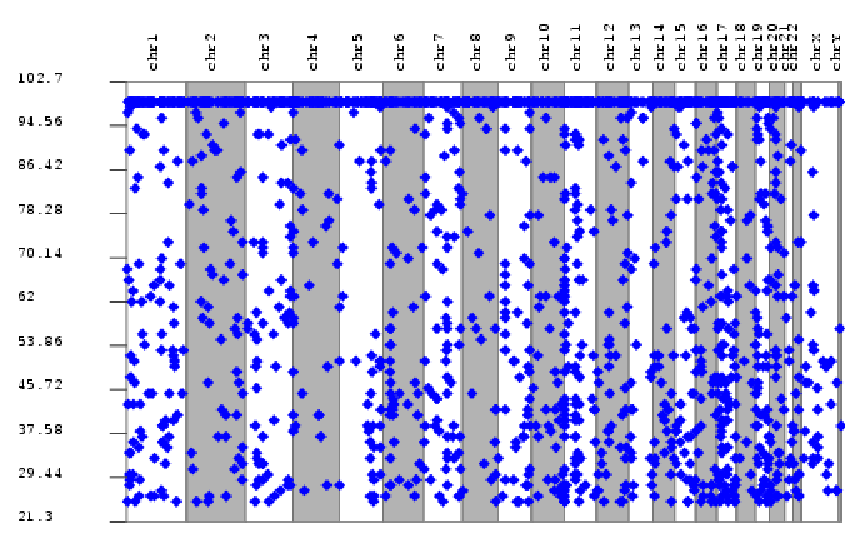
\includegraphics{manhattan.eps}
\caption{An Manhattan plot}
\end{figure}
\paragraph{Example2:}
plotting with Samples and Colors.
\begin{quote}
\begin{verbatim}
 cat sample2vcf.tsv |\
     scanvcf | awk '($3==".")' |grep NON_SYNO |\
     cut -d '     ' -f 1,2,6,11 |\
     awk '{printf("%s\trgb(10,%d,%d)\n",$0,255-(int($3)/100.0)*255.0,(int($3)/100.0)*255.0);}'|\
     manhattan -v 3 -r 5 -s 4 > result.ps
$ evince result.ps
\end{verbatim}
\end{quote}
\begin{figure}
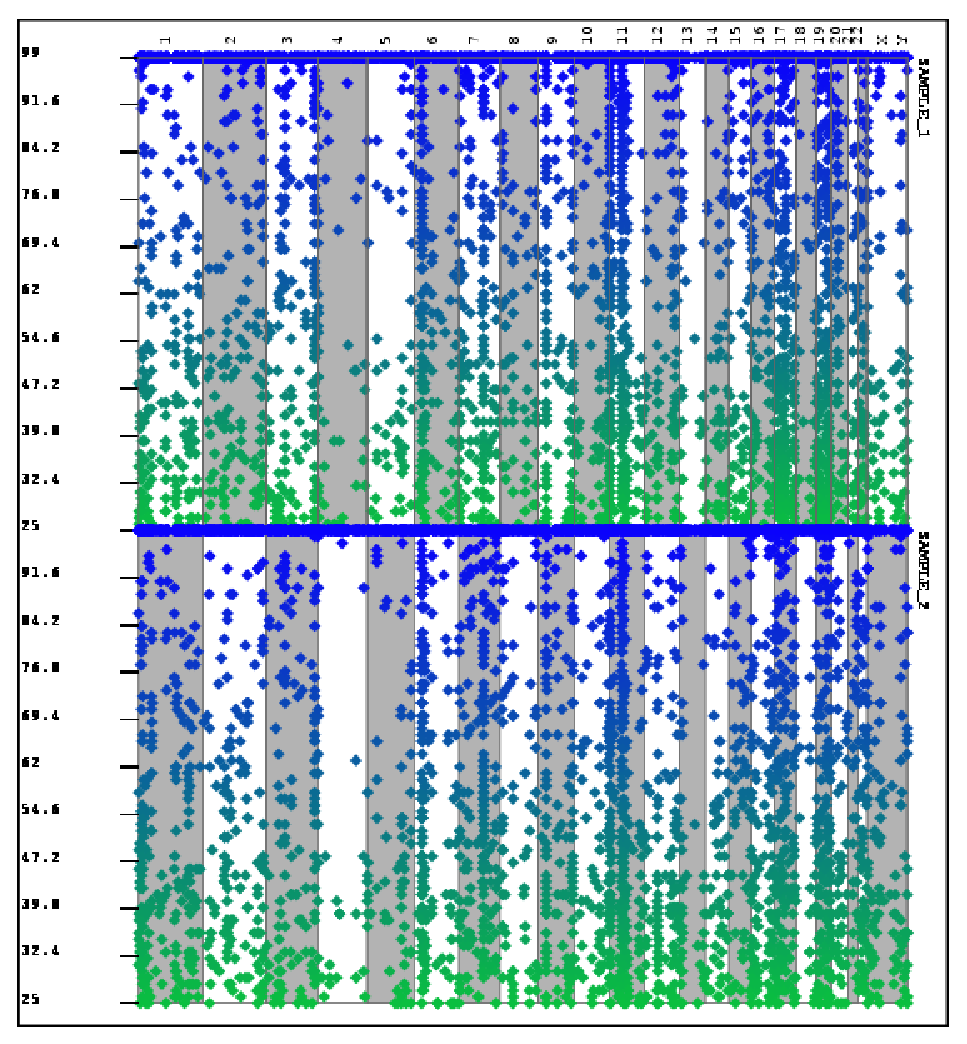
\includegraphics[keepaspectratio=true,scale=1.0]{manhattan2.eps}
\caption{An Manhattan plot with colors and samples}
\end{figure}

\subsection{ncbiesearch}
Search NCBI/Entrez:
\paragraph{Options:}
\begin{itemize}
\item-D (database) (default pubmed)
\item-q (query) [required]
\item-d (delimiter) (default:tab)
\item-L (limit=int) (default:10)
\end{itemize}
\paragraph{Example:}
The following example creates a sequence of 3 names, we search the NCBi for each name and the word "Rotavirus" in the title, limit to 2 record, we fetch each record (the PMID is in the 2nd column) and we cut the result down to 80 characters.
 
\begin{quote}
\begin{verbatim}
$ echo -e "#subject\nPiron\nLindenbaum\nPoncet" |\
   ncbiesearch -q '$1 "Rotavirus"[TITL]' -L 2  |\
   ncbiefetch -c 2 |\
   cut -c 1-80
#subject	pubmed.id	pubmed.year	pubmed.title	pubmed.journal	pubmed.abstract
Piron	10888646	2000	Efficient translation of rotavirus mRNA requires simultaneou
Piron	10364288	1999	Identification of the RNA-binding, dimerization, and eIF4GI-
Lindenbaum	15047801	2004	RoXaN, a novel cellular protein containing TPR, LD, and
Lindenbaum	8985320	1997	In vivo and in vitro phosphorylation of rotavirus NSP5 c
Poncet	21864538	2011	Structural Organisation of the Rotavirus Nonstructural Prot
Poncet	20935207	2010	Rapid generation of rotavirus-specific human monoclonal ant
\end{verbatim}
\end{quote}



\subsection{vcfttview}
Prints the BAM context around variations.
Original code from samtools ttview : Heng Li, Bob Handsaker, Jue Ruan, Colin Hercus, Petr Danecek
\paragraph{Options:}
\begin{itemize}
\item-c (chrom Column) (1)
\item-p (pos Column) (2)
\item-s (sample Column) (0) [optional]
\item-d (column-delimiter) (default:tab)
\item-B (bam-file) [defines one main bam for all data]
\item-f (file) loads a file tab delimited with SAMPLE-NAME\\tPATH-TO-BAM
\item-F (SAMPLE) (FILE)  push a SAMPLE-NAME/PATH-TO-BAM in the current list
\item-a for one position, print all BAM
\item-x (int) shift x bases to the right: default10
\item-w (int) screen width default:80
\item-R (fasta) reference file indexed with samtools faidx 
\end{itemize}
\paragraph{Example:}
\begin{quote}
\begin{verbatim}

$ echo -e "ref\t3\nref2\t2" |\
  vcfttview -x 3 -B toy.bam -R toy.fa

>ref:3

1         11              21        31         41        51        61           
AGCATGTTAGATAA****GATA**GCTGTGCTAGTAGGCAG*TCAGCGCCATNNNNNNNNNNNNNNNNNNNNNNNNNNNN
      ........    ....  ......K.K......K. ..........                            
      ........AGAG....***...      ,,,,,    ,,,,,,,,,                            
        ......GG**....AA                                                        
        ..C...**** ...**...>>>>>>>>>>>>>>T.....                                 



>ref2:2

1         11            21        31        41        51        61              
aggttttataaaac****aattaagtctacagagcaactacgcgNNNNNNNNNNNNNNNNNNNNNNNNNNNNNNNNNNNN
.............Y    ..W...................                                        
..............****..A...                                                        
 .............****..A...T.                                                      
     .........AAAT.............                                                 
         C...T****....................                                          
           ..T****.....................                                         
             T****......................                                        
                                                               
\end{verbatim}
\end{quote}

\subsection{vcftabix}
Intersection VCF/Tabix
\paragraph{Options:}
\begin{itemize}
\item-d (char) column delimiter. default: TAB
\item-c (int) chromosome column (1).
\item-p (int) pos column (2).
\item-f (filename) tabix file (required).
\item-1 remove 1 to the VCF coodinates.
\item-S (NOT-FOUND-String) default:!N/A.
\item-m  (int=mode) 0)=all 1:only-matching  2:only-non-matching default:0.
\end{itemize}
\paragraph{Example:}
 download some 1000G data:
\begin{quote}
\begin{verbatim}
 curl  -s "ftp://ftp-trace.ncbi.nih.gov/1000genomes/ftp/release/20100804/ALL.2of4intersection.20100804.sites.vcf.gz" |\
            gunzip -c | grep -v "##" |\
            head -n 10000 > ~/1000G.vcf
\end{verbatim}
\end{quote}
Index this file with tabix.
\begin{quote}
\begin{verbatim}
$ bgzip 1000G.vcf
$ tabix -p vcf 1000G.vcf.gz
\begin{verbatim}
\end{verbatim}
\end{quote}
Compute the intersection of this file with our VCF. Only retain the matching line (option -m 1)
\begin{quote}
\begin{verbatim}
$ gunzip -c data.vcf.gz |\
  grep -v "##"  |  normalizechrom -E | vcftabix  -f 1000G.vcf.gz -m 1 |\
  awk '($8=".")' |  awk '($18=".")'
#CHROM POS ID REF ALT QUAL FILTER . FORMAT Call #CHROM POS ID REF ALT QUAL FILTER .
1 879317 rs7523549 C T 71 0 . GT:GQ:DP:FLT 0/1:34:8:0 1 879317 rs7523549 C T . PASS .
1 880238 rs3748592 A G 51 0 . GT:GQ:DP:FLT 1/1:51:8:0 1 880238 rs3748592 A G . PASS .
1 880390 rs3748593 C A 99 0 . GT:GQ:DP:FLT 1/0:99:30:0 1 880390 rs3748593 C A . PASS .
1 881627 rs2272757 G A 99 0 . GT:GQ:DP:FLT 1/0:59:20:0 1 881627 rs2272757 G A . PASS .
1 883625 rs4970378 A G 39 0 . GT:GQ:DP:FLT 1/1:39:4:0 1 883625 rs4970378 A G . PASS .
1 887560 rs3748595 A C 99 0 . GT:GQ:DP:FLT 1/1:99:40:0 1 887560 rs3748595 A C . PASS .
1 887801 rs3828047 A G 99 0 . GT:GQ:DP:FLT 1/1:99:32:0 1 887801 rs3828047 A G . PASS .
1 888639 rs3748596 T C 99 0 . GT:GQ:DP:FLT 1/1:99:32:0 1 888639 rs3748596 T C . PASS .
1 888659 rs3748597 T C 99 0 . GT:GQ:DP:FLT 1/1:99:26:0 1 888659 rs3748597 T C . PASS .
(...)
\end{verbatim}
\end{quote}


\subsection{mysqlquery}
Sends a mysql query for each row:
\paragraph{Options:}
\begin{itemize}
\item-d (char) delimiter default:tab
\item--host mysql host ( genome-mysql.cse.ucsc.edu)
\item--user mysql user ( genome)
\item--password mysql password ( )
\item--database mysql db ( hg19)
\item--port (int) mysql port ( default)
\item-e or -q (SQL query)
\item-L (int) limit number or rows returned
\end{itemize}
\paragraph{Example:}

\begin{quote}
\begin{verbatim}
$  echo -e "#Gene\nuc001aaa.3\nHello\nuc001aac.3" |\
      mysqlquery --host localhost --user anonymous --port 3316  \
             -q 'select mRNA,description from kgXref where kgId="$1"'  |\
      verticalize 
>>>	2
$1	#Gene      	uc001aaa.3
$2	mRNA       	BC032353
$3	description	Homo sapiens mRNA for DEAD/H box polypeptide 11 like 1 (DDX11L1 gene).
<<<	2

>>>	3
$1	#Gene      	Hello
$2	mRNA       	.
$3	description	.
<<<	3

>>>	4
$1	#Gene      	uc001aac.3
$2	mRNA       	BC063459
$3	description	Homo sapiens cDNA FLJ31670 fis, clone NT2RI2004984.
<<<	4
\end{verbatim}
\end{quote}

\subsection{mysqlucsc}
Intersection VCF/UCSC mysql data.
\paragraph{Options:}
\begin{itemize}
\item--delim (char) delimiter default:tab
\item--host mysql host ( genome-mysql.cse.ucsc.edu)
\item--user mysql user ( genome)
\item--password mysql password ( )
\item--database mysql db ( hg19)
\item--port (int) mysql port ( default)
\item--table or -T (string)
\item-C (int) chromosome column (first is 1).
\item-S (int)start column (first is 1).
\item-E (int) end column (first is 1).
\item-f first column is not header.
\item-1 data are +1 based.
\item--limit (int) limit number or rows returned
\item--field (string) set custom field. Can be used several times
\item--type (int) type of selection: 0 any (default), 1 user data IN mysql data,2 user data embrace mysql data. (stdin|files)
\end{itemize}
\paragraph{Example:}
Compute the intersection of our data with ucsc.snp132 keep the lines containing the word 'syn'.
\begin{quote}
\begin{verbatim}
$ gunzip -c data.vcf.gz |\
   grep -v "##"  |  normalizechrom |\
   mysqlucsc --host myhost --user mypassword -C 1 -S 2 -E 2 --table snp132    |\
   awk '($8=".")' | grep -i syn |\
   head
   
chr1 16375063 rs45612832 C G 67 0 . GT:GQ:DP:FLT 0/1:67:53:0 709 chr1 16375063 16375064 rs1889790 0 + A A A/C genomic single by-cluster,by-frequency 0.4488 0.151587 coding-synon,near-gene-5 exact 1 NonIntegerChromCount 9 BCMHGSC_JDW,BCM_SSAHASNP,BGI,HGSV,SC_SNP,SEATTLESEQ,SSAHASNP,TSC-CSHL,UCSF_HG, 2 A,C, 15.980000,31.020000, 0.340000,0.660000, maf-5-some-pop,maf-5-all-pops
chr1 16375063 rs45612832 C G 67 0 . GT:GQ:DP:FLT 0/1:67:53:0 709 chr1 16375063 16375064 rs45575235 0 + A A A/C genomic single by-cluster,by-frequency 0 0 coding-synon,near-gene-5 exact 2 MultipleAlignments 3 ENSEMBL,GMI,PHARMGKB_PCE, 1 C, 2.000000, 1.000000, maf-5-some-pop,maf-5-all-pops
chr1 16890671 rs55951643 T C 99 0 . GT:GQ:DP:FLT 1/0:99:1177:0 713 chr1 16890671 16890672 rs2419525 0 - G G C/T genomic single by-cluster,by-2hit-2allele,by-hapmap 0.18 0.24 coding-synon exact 1 10 BCMHGSC_JDW,BGI,CSHL-HAPMAP,ENSEMBL,GMI,HGSV,SC_JCM,SC_SNP,TSC-CSHL,WI_SSAHASNP, 2 T,C, 9.000000,1.000000, 0.900000,0.100000, maf-5-some-pop,maf-5-all-pops
chr1 16890671 rs55951643 T C 99 0 . GT:GQ:DP:FLT 1/0:99:1177:0 713 chr1 16890671 16890672 rs17409315 0 - G G C/T cDNA single unknown 0 0 coding-synon exact 3 MultipleAlignments 1 SEQUENOM, 0
chr1 22176831 rs2290500 C T 87 0 . GT:GQ:DP:FLT 0/1:47:9:0 754 chr1 22176683 22176855 rs2229485 0 - TGCTGGGGACAGAGGGCAAAGGGTCAATAGCCGGCTAGGAGGTGAGATGAGATGGGGCTCCTGGTCTCAAGGCAGGTGCAGTCTGCGGCTTGGCCTCCTGATCCTGCCGTTGCAAGAGTGGGGGGCCTCCCACCCTGGGTCCCCAGCCCTGCCCTCCCTGAGAGCTACTCAC TGCTGGGGACAGAGGGCAAAGGGTCAATAGCCGGCTAGGAGGTGAGATGAGATGGGGCTCCTGGTCTCAAGGCAGGTGCAGTCTGCGGCTTGGCCTCCTGATCCTGCCGTTGCAAGAGTGGGGGGCCTCCCACCCTGGGTCCCCAGCCCTGCCCTCCCTGAGAGCTACTCAC A/T cDNA single by-frequency 0.120708 0.213971 coding-synon rangeInsertion 1 FlankMismatchGenomeLonger,SingleClassLongerSpan,ObservedMismatch 2 CORNELL,WICVAR, 2 T,A, 77.000000,59.000000, 0.566176,0.433824, maf-5-some-pop,maf-5-all-pops,observed-mismatch
chr1 26361669 rs61742342 C A 99 0 . GT:GQ:DP:FLT 1/0:99:34:0 786 chr1 26361669 26361670 rs61739493 0 + G G G/T genomic single unknown 0 0 coding-synon exact 1 1 CORNELL, 2 G,T, 77.000000,1.000000, 0.987179,0.012820,
chr1 26608828 rs17838088 G A 36 0 . GT:GQ:DP:FLT 1/1:28:4:0 788 chr1 26608828 26608829 rs61775085 0 + G G A/G genomic single unknown 0.5 0 coding-synon exact 1 2 BCMHGSC_JDW,ENSEMBL, 2 G,A, 1.000000,1.000000, 0.500000,0.500000, maf-5-some-pop,maf-5-all-pops
chr1 27210721 rs3170660 T C 99 0 . GT:GQ:DP:FLT 1/1:99:63:0 792 chr1 27210721 27210722 rs78109142 0 + G G A/G genomic single by-cluster,by-frequency,by-1000genomes 0.165289 0.235211 coding-synon exact 1 1 1000GENOMES, 2 G,A, 195.000000,13.000000, 0.937500,0.062500, maf-5-some-pop,maf-5-all-pops
chr1 64643277 rs7527017 C T 99 0 . GT:GQ:DP:FLT 0/1:99:117:0 1078 chr1 64643277 64643278 rs80063252 0 + G G A/G genomic single by-cluster,by-frequency,by-1000genomes 0.0768 0.180282 coding-synon exact 1 1 1000GENOMES, 2 G,A, 158.000000,10.000000, 0.940476,0.059524, maf-5-some-pop
chr1 110709719 rs7527375 T C 99 0 . GT:GQ:DP:FLT 1/0:99:31:0 1429 chr1 110709719 110709720 rs12737742 0 + G G A/C/G genomic single by-cluster,by-1000genomes 0.375 0.216506 coding-synon,missense exact 1 SingleClassTriAllelic 9 1000GENOMES,BCMHGSC_JDW,BUSHMAN,CORNELL,ENSEMBL,HGSV,ILLUMINA,SEATTLESEQ,SSAHASNP, 3 G,A,C, 57.000000,21.000000,1.000000, 0.721519,0.265823,0.012658, maf-5-some-pop,maf-5-all-pops
\end{verbatim}
\end{quote}

\subsection{vcfbigwig}
Intersection VCF/BigWig
\paragraph{Options:}
\begin{itemize}
\item-f (bigwig file)
\item-d (delimiter) (default:tab)
\item-c (CHROM column=int) (default:1)
\item-p (POS column=int) (default:2)
\item-x (extend=int) extends window size (default:0)
\end{itemize}
\paragraph{Example:}
What's in the Big wig ?
\begin{quote}
\begin{verbatim}
$ kent/src/hg/encode/validateFiles/tests/test4.bw file.wig
$ cat file.wig

#bedGraph section chr1:1-1099
chr1    1       1000    54
chr1    1000    1099    53
\end{verbatim}
\end{quote}

let's get the intersection of a VCF file with this BIGWIG file.

\begin{quote}
\begin{verbatim}
$ echo -e "#CHROM\tPOS\nchr1\t500\nchr1\t1001"  |\
  vcfbigwig -f  kent/src/hg/encode/validateFiles/tests/test4.bw
  
#CHROM	POS	bigwig:min	bigwig:max	bigwig:mean	bigwig:coverage	bigwig:stddev
chr1	500	54	54	54	1	0
chr1	1001	53	53	53	1	0

$ echo -e "#CHROM\tPOS\nchr1\t500\nchr1\t1001"  |\
  vcfbigwig -x 100 -f  kent/src/hg/encode/validateFiles/tests/test4.bw
  
#CHROM	POS	bigwig:min	bigwig:max	bigwig:mean	bigwig:coverage	bigwig:stddev
chr1	500	54	54	54	1	0
chr1	1001	53	54	53.5025	0.99005	0.501255

$ echo -e "#CHROM\tPOS\nchrX\t500\nchrX\t1001"  |\
  vcfbigwig  -f  kent/src/hg/encode/validateFiles/tests/test4.bw
  
#CHROM	POS	bigwig:min	bigwig:max	bigwig:mean	bigwig:coverage	bigwig:stddev
chrX	500	nan	nan	nan	nan	nan
chrX	1001	nan	nan	nan	nan	nan
\end{verbatim}
\end{quote}

\subsection{vcfbigbed}
Intersection VCF/BigBed
\paragraph{Options:}
\begin{itemize}
\item-f (BigBed file)
\item-d (delimiter) (default:tab)
\item-c (CHROM column=int) (default:1)
\item-p (POS column=int) (default:2)
\item-x (extend=int) extends window size (default:0)
\item-L (limit=int) limit to L records in bed (default:unbound)
\item-S (NOT-FOUND-String) default:!N/A.
\item-m  (int=mode) 0)=all 1:only-matching  2:only-non-matching default:0.
\end{itemize}
\paragraph{Example:}
What's in the Big BED ?
\begin{quote}
\begin{verbatim}
$ cat test.bed 
chr7    115000000       116000000       100.0
chr7    115500000       116500000       200.0
chr7    116000000       117000000       100.0
chr8    1000000         2000000         1000
chr8    1100000         1200000         1000
chr8    1100000         1200000         1000
chr9    100     200     10
chr9    100     300     10
chr9    100     400     10
chr9    1000    2000    10
chr9    1200    2000    10
chr9    1300    2000    10
\end{verbatim}
\end{quote}

let's get the intersection of a VCF file with this BigBed file.

\begin{quote}
\begin{verbatim}
$ echo -e "#CHROM\tPOS\nchr9\t1250\nchrX\t1"  |\
  vcfbigbed  -f  test.bb 

#CHROM	POS	BigBed:chromStart	BigBed:chromEnd	BigBed:rest
chr9	1250	1000	2000	10
chr9	1250	1200	2000	10
chrX	1	!N/A	!N/A	!N/A

$ echo -e "#CHROM\tPOS\nchr9\t1250\nchrX\t1"  |\
  vcfbigbed  -x 1000 -f  test.bb 

#CHROM	POS	BigBed:chromStart	BigBed:chromEnd	BigBed:rest
chr9	1250	100	300	10
chr9	1250	100	400	10
chr9	1250	1000	2000	10
chr9	1250	1200	2000	10
chr9	1250	1300	2000	10
chrX	1	!N/A	!N/A	!N/A

\end{verbatim}
\end{quote}

\subsection{verticalize}
Verticalize a table.
\paragraph{Options:}
\begin{itemize}
\item-d or --delim (char) delimiter default:tab
\item-n first line is NOT the header.
\end{itemize}
\paragraph{Example:}
\begin{quote}
\begin{verbatim}
$ gunzip -c file.vcf.gz | grep -v "##" |\
   verticalize  |\
   head -n 100
>>>	2
$1	#CHROM   	1
$2	POS      	880238
$3	ID       	rs3748592
$4	REF      	A
$5	ALT      	G
$6	QUAL     	48
$7	FILTER   	0
$8	INFO     	AC=2;DB=1;ST=0:0,3:4;DP=7;NC=-3.73;UM=3;CQ=INTRONIC;MQ=60;AN=2;PA=1^1:0.930&2^1:0.860&3^1:0.950;MZ=0;GN=NOC2L;PS=1
$9	FORMAT   	GT:GQ:DP:FLT
$10	162214_A1	1/1:48:7:0
<<<	2

>>>	3
$1	#CHROM   	1
(...)
\end{verbatim}
\end{quote}

\subsection{uniprot}
Take as input a position on a protein and an uniprot ACN, connect to uniprot.org and answers wether a amino acid is contained in a 'feature'.
\paragraph{Options:}
\begin{itemize}
\item-d (char) delimiter default:tab
\item-p (column-index) column containing the amino acid index.
\item-s (spId-index) column containing the swissprot-acn  (e.g.: Q04721 or  NOTC2\_HUMAN).
\end{itemize}
\paragraph{Example:}

\begin{quote}
\begin{verbatim}
$ echo -e "#POS\tID\n54\tQ04721\n1\tHELLO\n166\tP03536" |\
    uniprot -p 1 -s 2 |\
    verticalize 
#warning: Cannot find record for HELLO
>>>	2
$1	#POS            	54
$2	ID              	Q04721
$3	uniprot.beg     	26
$4	uniprot.end     	2471
$5	uniprot.type    	chain
$6	uniprot.status  	.
$7	uniprot.desc    	Neurogenic locus notch homolog protein 2
$8	uniprot.evidence	.
$9	uniprot.ref     	.
<<<	2

>>>	3
$1	#POS            	54
$2	ID              	Q04721
$3	uniprot.beg     	26
$4	uniprot.end     	1677
$5	uniprot.type    	topological domain
$6	uniprot.status  	potential
$7	uniprot.desc    	Extracellular
$8	uniprot.evidence	.
$9	uniprot.ref     	.
<<<	3

>>>	4
$1	#POS            	54
$2	ID              	Q04721
$3	uniprot.beg     	26
$4	uniprot.end     	63
$5	uniprot.type    	domain
$6	uniprot.status  	.
$7	uniprot.desc    	EGF-like 1
$8	uniprot.evidence	.
$9	uniprot.ref     	.
<<<	4

>>>	5
$1	#POS            	54
$2	ID              	Q04721
$3	uniprot.beg     	53
$4	uniprot.end     	62
$5	uniprot.type    	disulfide bond
$6	uniprot.status  	by similarity
$7	uniprot.desc    	.
$8	uniprot.evidence	.
$9	uniprot.ref     	.
<<<	5

>>>	6
$1	#POS            	1
$2	ID              	HELLO
$3	uniprot.beg     	.
$4	uniprot.end     	.
$5	uniprot.type    	.
$6	uniprot.status  	.
$7	uniprot.desc    	.
$8	uniprot.evidence	.
$9	uniprot.ref     	.
<<<	6

>>>	7
$1	#POS            	166
$2	ID              	P03536
$3	uniprot.beg     	1
$4	uniprot.end     	315
$5	uniprot.type    	chain
$6	uniprot.status  	.
$7	uniprot.desc    	Non-structural protein 3
$8	uniprot.evidence	.
$9	uniprot.ref     	.
<<<	7

>>>	8
$1	#POS            	166
$2	ID              	P03536
$3	uniprot.beg     	150
$4	uniprot.end     	206
$5	uniprot.type    	region of interest
$6	uniprot.status  	.
$7	uniprot.desc    	Dimerization
$8	uniprot.evidence	.
$9	uniprot.ref     	.
<<<	8

>>>	9
$1	#POS            	166
$2	ID              	P03536
$3	uniprot.beg     	166
$4	uniprot.end     	237
$5	uniprot.type    	coiled-coil region
$6	uniprot.status  	potential
$7	uniprot.desc    	.
$8	uniprot.evidence	.
$9	uniprot.ref     	.
<<<	9
\end{verbatim}
\end{quote}


\subsection{pfamscan}
Take as input a position on a protein and an uniprot ACN, connect to  pfam.sanger.ac.uk and answers wether a amino acid is contained in a 'match'.
\paragraph{Options:}
\begin{itemize}
\item-d (char) delimiter default:tab
\item-p (column-index) column containing the amino acid index.
\item-a (acn) column containing the protein-acn (e.g.: Q04721 or  IF4G1\_HUMAN).
\end{itemize}
\paragraph{Example:}
\begin{quote}
\begin{verbatim}
$ echo -e "#ACN\tPOS\nQ04721\t1650\nIF4G1_HUMAN\t1540\nQ04721\t300\nHello\t9980\n.\t." |\
	pfamscan -a 1 -p 2 |\
	verticalize


>>>	2
$1	#ACN      	Q04721
$2	POS       	1650
$3	pfam.beg  	1617
$4	pfam.end  	1677
$5	pfam.acn  	PF07684
$6	pfam.id   	NODP
$7	pfam.type 	Pfam-A
$8	pfam.class	.
<<<	2

>>>	3
$1	#ACN      	IF4G1_HUMAN
$2	POS       	1540
$3	pfam.beg  	1518
$4	pfam.end  	1599
$5	pfam.acn  	PF02020
$6	pfam.id   	W2
$7	pfam.type 	Pfam-A
$8	pfam.class	.
<<<	3

>>>	4
$1	#ACN      	Q04721
$2	POS       	300
$3	pfam.beg  	298
$4	pfam.end  	338
$5	pfam.acn  	PF07645
$6	pfam.id   	EGF_CA
$7	pfam.type 	Pfam-A
$8	pfam.class	.
<<<	4

>>>	5
$1	#ACN      	Hello
$2	POS       	9980
$3	pfam.beg  	.
$4	pfam.end  	.
$5	pfam.acn  	.
$6	pfam.id   	.
$7	pfam.type 	.
$8	pfam.class	.
<<<	5

>>>	6
$1	#ACN      	.
$2	POS       	.
$3	pfam.beg  	.
$4	pfam.end  	.
$5	pfam.acn  	.
$6	pfam.id   	.
$7	pfam.type 	.
$8	pfam.class	.
<<<	6
\end{verbatim}
\end{quote}


\subsection{vcf2bed}
Generates a BED file from a VCF.

\paragraph{Options:}
\begin{itemize}
\item-d (column-delimiter) (default:tab)
\item-c (CHROM col) (default:0)
\item-p (POS col) (default:1)
\item-S (bed score col) (default:-1)
\item-N (col) adds this column for the 'name'
\item-D (char) name separator.
\item-t print ucsc custom track header.
\end{itemize}
\paragraph{Example:}

\begin{quote}
\begin{verbatim}
$ gunzip -c file.vcf.gz |\
  normalizechrom |\
  vcf2bed -t -S 6 -N 3,4,5 -D _

track name="__TRACK_NAME__" description="__TRACK_DESC__" 
chr1	879316	879317	rs7523549_C_T	71	+
chr1	880237	880238	rs3748592_A_G	51	+
chr1	880389	880390	rs3748593_C_A	99	+
chr1	881626	881627	rs2272757_G_A	99	+
chr1	883624	883625	rs4970378_A_G	39	+
chr1	887559	887560	rs3748595_A_C	99	+
chr1	887800	887801	rs3828047_A_G	99	+
chr1	888638	888639	rs3748596_T_C	99	+
chr1	888658	888659	rs3748597_T_C	99	+
chr1	889157	889158	rs56262069_G_C	51	+
(...)
\end{verbatim}
\end{quote}

\subsection{emblstringresolve}
Calls the service: EMBL String resolve ( \url{http://string-db.org/help/index.jsp?topic=/org.string-db.docs/api.html} ).

\paragraph{Options:}
\begin{itemize}
\item-d (char) delimiter default:tab
\item-c column identifier
\item-t (int) taxon id
\end{itemize}
\paragraph{Example:}


\begin{quote}
\begin{verbatim}
$ echo -e "#Gene\nNOTCH2\nEIF4G1\nPABPC1" |\
  emblstringresolve -c 1 |verticalize 
>>>	2
$1	#Gene        	NOTCH2
$2	stringId     	9606.ENSP00000256646
$3	preferredName	NOTCH2
$4	annotation   	Notch homolog 2 (Drosophila); Functions as a receptor...
<<<	2

>>>	3
$1	#Gene        	EIF4G1
$2	stringId     	9606.ENSP00000316879
$3	preferredName	EIF4G1
$4	annotation   	eukaryotic translation initiation factor 4 gamma, 1; ...
<<<	3

>>>	4
$1	#Gene        	PABPC1
$2	stringId     	9606.ENSP00000313007
$3	preferredName	PABPC1
$4	annotation   	poly(A) binding protein, cytoplasmic 1; Binds the...
<<<	4
\end{verbatim}
\end{quote}


\subsection{emblstringinteractors}
Calls the service: EMBL String interactors ( \url{http://string-db.org/help/index.jsp?topic=/org.string-db.docs/api.html} ).


\paragraph{Options:}
\begin{itemize}
\item-d (char) delimiter default:tab
\item-c column identifier
\end{itemize}
\paragraph{Example:}

\begin{quote}
\begin{verbatim}
$ echo -e "#Gene\nNOTCH2\nEIF4G1\nPABPC1" |\
  emblstringresolve -c 1 | \
  emblstringinteractors -c 2 | \
  emblstringresolve -c 5 | \
  verticalize
  
>>>	2
$1	#Gene        	NOTCH2
$2	stringId     	9606.ENSP00000256646
$3	preferredName	NOTCH2
$4	annotation   	Notch homolog 2 (Drosophila); Functions as a receptor for membr
$5	interactor   	9606.ENSP00000256646
$6	stringId     	9606.ENSP00000256646
$7	preferredName	NOTCH2
$8	annotation   	Notch homolog 2 (Drosophila); Functions as a receptor for membr
<<<	2

>>>	3
$1	#Gene        	NOTCH2
$2	stringId     	9606.ENSP00000256646
$3	preferredName	NOTCH2
$4	annotation   	Notch homolog 2 (Drosophila); Functions as a receptor for membr
$5	interactor   	9606.ENSP00000345206
$6	stringId     	9606.ENSP00000345206
$7	preferredName	RBPJ
$8	annotation   	recombination signal binding protein for immunoglobulin kappa J
<<<	3

>>>	4
$1	#Gene        	NOTCH2
$2	stringId     	9606.ENSP00000256646
$3	preferredName	NOTCH2
$4	annotation   	Notch homolog 2 (Drosophila); Functions as a receptor for membr
$5	interactor   	9606.ENSP00000355718
$6	stringId     	9606.ENSP00000355718
$7	preferredName	DLL1
  
  
\end{verbatim}
\end{quote}

\subsection{emblstringinteractions}
Calls the service: EMBL String interactions ( \url{http://string-db.org/help/index.jsp?topic=/org.string-db.docs/api.html} ).
\paragraph{Options:}
\begin{itemize}
\item-d (char) delimiter default:tab
\item-c column identifier
\end{itemize}
\paragraph{Example:}
\begin{quote}
\begin{verbatim}
$ echo -e "#Gene\nNOTCH2\nEIF4G1\nPABPC1" | \
   emblstringresolve -c 1 | \
   emblstringinteractions -c 2 | \
   verticalize 
   
>>>	2
$1	#Gene          	NOTCH2
$2	stringId       	9606.ENSP00000256646
$3	preferredName  	NOTCH2
$4	annotation     	Notch homolog 2 (Drosophila); Functions as a receptor for membrane-bound ligands Jagged1, Jagged2 and Delta1 to regulate cell-fate determination. Upon ligand activation through the released notch intracellular domain (NICD) it forms a transcriptional activator complex with RBP-J kappa and activates genes of the enhancer of split locus. Affects the implementation of differentiation, proliferation and apoptotic programs (By similarity)
$5	interactorA    	string:9606.ENSP00000355718
$6	interactorB    	string:9606.ENSP00000326366
$7	labelA         	DLL1
$8	labelB         	PSEN1
$9	aliasesA       	-
$10	aliasesB       	-
$11	method         	-
$12	firstAuthor    	-
$13	publication    	-
$14	taxonA         	taxid:9606
$15	taxonB         	taxid:9606
$16	types          	-
$17	sources        	-
$18	interaction.ids	-
$19	score          	score:0.999|escore:0.639|dscore:0.9|tscore:0.984
<<<	2

>>>	3
$1	#Gene          	NOTCH2
$2	stringId       	9606.ENSP00000256646
$3	preferredName  	NOTCH2
$4	annotation     	Notch homolog 2 (Drosophila); Functions as a receptor for membrane-bound ligands Jagged1, Jagged2 and Delta1 to regulate cell-fate determination. Upon ligand activation through the released notch intracellular domain (NICD) it forms a transcriptional activator complex with RBP-J kappa and activates genes of the enhancer of split locus. Affects the implementation of differentiation, proliferation and apoptotic programs (By similarity)
$5	interactorA    	string:9606.ENSP00000345206
$6	interactorB    	string:9606.ENSP00000292599
$7	labelA         	RBPJ

\end{verbatim}
\end{quote}

\subsection{vcfcut}
Simple "cut this region".
\begin{quote}
\begin{verbatim}
$ curl -s "ftp://ftp-trace.ncbi.nih.gov/1000genomes/ftp/release/20100804/ALL.2of4intersection.20100804.sites.vcf.gz" |\
   gunzip -c | grep -v "##" |\
   vcfcut -e '2:10kb+500bp;1:10000-20000'
   
#CHROM	POS	ID	REF	ALT	QUAL	FILTER	INFO
1	10327	rs112750067	T	C	.	PASS	DP=65;AF=0.208;CB=BC,NCBI
1	10469	rs117577454	C	G	.	PASS	DP=2055;AF=0.020;CB=UM,BC,NCBI
1	10492	rs55998931	C	T	.	PASS	DP=231;AF=0.167;CB=BC,NCBI
(...)
1	16841	.	G	T	.	PASS	DP=2906;AF=0.004;CB=UM,BI;EUR_R2=0.248
2	10038	.	C	A	.	PASS	DP=73;AF=0.409;CB=BC,NCBI
2	10075	.	C	A	.	PASS	DP=31;AF=0.150;CB=BC,NCBI
2	10144	.	C	A	.	PASS	DP=33;AF=0.562;CB=BC,NCBI
2	10159	.	C	A	.	PASS	DP=32;AF=0.222;CB=BC,NCBI
2	10205	.	T	G	.	PASS	DP=582;AF=0.107;CB=UM,BC
2	10297	.	G	T	.	PASS	DP=500;AF=0.246;CB=UM,BC
2	10363	.	G	A	.	PASS	DP=788;AF=0.016;CB=UM,BI;EUR_R2=0.273;AFR_R2=0.034
2	10437	rs71337607	C	T	.	PASS	DP=324;AF=0.267;CB=UM,BC
\end{verbatim}
\end{quote}

\subsection{ucscgenesps}
Reads an ordered VCF (ordered by CHROM/POS and optionaly by SAMPLE) , connect to an UCSC database a print the
variation in postscript.
\paragraph{Options:}
\begin{itemize}
\item-c (int) CHROM column default:1
\item-p (int) POS column default:2
\item-s (int) SAMPLE column (optional) 
\item-r (int) COLOR column (optional)
\item--host (mysql host) default:genome-mysql.cse.ucsc.edu
\item--user (mysql user) default:genome
\item--password (mysql password) default:
\item--database (mysql database) default:hg19
\item--port (mysql password) default:0
\end{itemize}
\paragraph{Example:}
\begin{figure}
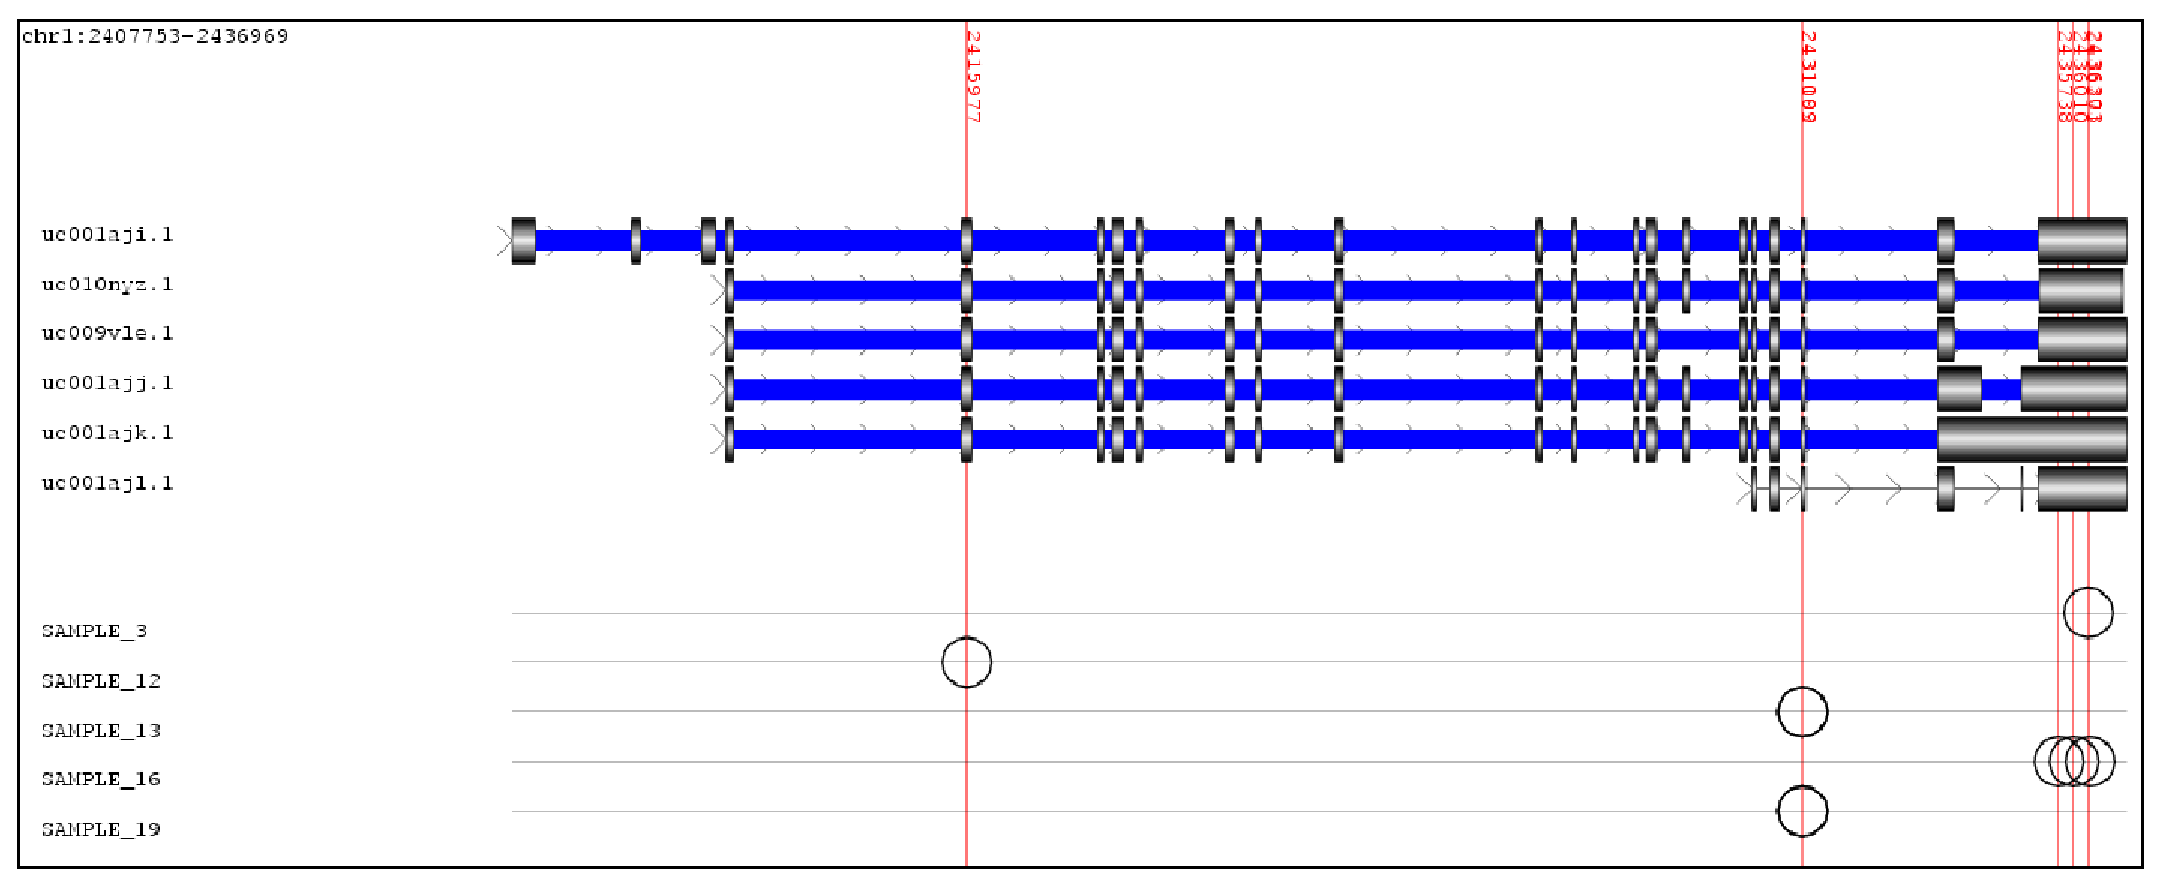
\includegraphics[keepaspectratio=true,scale=0.45]{ucscgenes.eps}
\caption{Structure of a gene}
\end{figure}
\begin{quote}
\begin{verbatim}
$ cat sample2vcf.tsv | tr -d ' ' |\
  scanvcf |\
  awk -F '      ' '($3==".")' |\
  normalizechrom |\
  sort -t '  ' -k1,1 -k2,2n -k11,11 |\
  head -n 10000 |\
  ucscgenesps --host localhost --user username --port 3316 -s 11 > result.ps 
\end{verbatim}
\end{quote}


\subsection{vcfintersect}
Compute the intersection for an ordered VCF (ordered by CHROM/POS) with another source ordered by CHROM/POS.
\paragraph{Options:}
\begin{itemize}
\item-f <external url/file> [required]
\item-m (mode) 0:all 1:matching 2:unmatching default:0
\item-n (string) no-match string default: NO\_MATCH
\item-c1 (CHROM col) (default:1)
\item-s1 (START col) (default:2)
\item-e1 (END col) (default:2)
\item-d1 (delimiter) (default:tab)
\item-h1  toggle: input is half open (default:0)
\item-z1  toggle: input zero-based (default:0)
\item-c2 (CHROM col) (default:1)
\item-s2 (START col) (default:2)
\item-e2 (END col) (default:2)
\item-d2 (delimiter) (default:tab)
\item-h2  toggle: input is half open (default:1)
\item-z2  toggle: input zero-based (default:1)
\item--http  force database is a URL 
\item--gunzip  force database is a gzipped stream 
\end{itemize}
\paragraph{Example:}
annotate a VCF with the data from snp132 at the UCSC.
\begin{quote}
\begin{verbatim}
$ echo -e "#CHROM\tPOS\nchr1\t10519\nchr1\t10520\nchr1\t10828"|\
	vcfintersect -n NO\_MATCH -c2 2 -s2 3 -e2 4  \
		-f "http://hgdownload.cse.ucsc.edu/goldenPath/hg19/database/snp132.txt.gz" |\
	verticalize -n

>>>	1
$1  	#CHROM
$2  	POS
<<<	1

>>>	2
$1  	chr1
$2  	10519
$3  	585
$4  	chr1
$5  	10518
$6  	10519
$7  	rs62636508
$8  	0
$9  	+
$10 	G
$11 	G
$12 	C/G
$13 	genomic
$14 	single
$15 	by-1000genomes
$16 	0
$17 	0
$18 	unknown
$19 	exact
$20 	1
$21 	
$22 	2
$23 	1000GENOMES,BCMHGSC_JDW,
$24 	2
$25 	G,C,
$26 	112.000000,8.000000,
$27 	0.933333,0.066667,
$28 	
<<<	2

>>>	3
$1  	chr1
$2  	10520
$3  	NO_MATCH
<<<	3

>>>	4
$1  	chr1
$2  	10828
$3  	585
$4  	chr1
$5  	10827
$6  	10828
$7  	rs10218492
$8  	0
$9  	+
$10 	G
$11 	G
$12 	A/G
$13 	genomic
$14 	single
$15 	by-cluster
$16 	0
$17 	0
$18 	unknown
$19 	exact
$20 	1
$21 	
$22 	1
$23 	WUGSC_SSAHASNP,
$24 	0
$25 	
$26 	
$27 	
$28 	
<<<	4
\end{verbatim}
\end{quote}


\bibliographystyle{abbrv}
\bibliography{varkit}

\end{document}
